\section{Introducción y objetivos}


\begin{frame}[c]{Motivación}

    El comportamiento de las enfermedades infecciosas es especialmente relevante en países menos desarrollados, pues sufren consecuencias más graves.
    \\~\\
    Los modelos matemáticos en epidemiología ayudan a comprender los mecanismos que intervienen en la propagación de las enfermedades y sugerir mecanismos para su control.

\end{frame}


\begin{frame}{Objetivos}

    \begin{itemize}
        \item Marcados al inicio:

        \pause
        \begin{itemize}
            \item Descripción y estudio de modelos discretos en epidemiología.
            \pause
            \item Visualización del comportamiento de los modelos.
            \pause
            \item Desarrollo de una página web.
        \end{itemize}
        
        \pause
        \item Adicionales:

        \pause
        \begin{itemize}
            \item Descripción y estudio de modelos continuos en epidemiología.
            \pause
            \item Ajuste de datos a un modelo.
            \pause
            \item Estimación de parámetros en datos reales.
        \end{itemize}
    \end{itemize}

\end{frame}


%%%%%%%%%%%%%%%%%%%%%%%%%%%%%%%%%%%%%%%%%%


\section{Conceptos fundamentales}


\begin{frame}{Conceptos fundamentales (I)}

    \begin{block}{Epidemia}
        Las epidemias son brotes espontáneos de una enfermedad o situaciones endémicas, en las que la enfermedad está siempre presente.
    \end{block}  

    \pause

    En todos los modelos se parte de realizar las siguientes suposiciones \cite{allenDiscretetimeSISIR1994}:

    \begin{itemize}
        \item La población se mezcla de manera homogénea, es decir, todos los individuos tienen la misma probabilidad de interactuar entre ellos y contraer la enfermedad.
        \item El total de la población es constante y lo denotaremos por $N$.
    \end{itemize}

\end{frame}


\begin{frame}{Conceptos fundamentales (II)}

    \begin{block}{Individuos susceptibles (S)}
        Los individuos \textbf{susceptibles} son aquellos que pueden infectarse con la enfermedad pero aún no lo han hecho.
    \end{block}  

    \pause

    \begin{block}{Individuos infectados (I)}
        Los individuos \textbf{infectados} son las personas infectadas por la enfermedad y pueden contagiar la enfermedad a los individuos susceptibles.
    \end{block}  

    \pause

    \begin{block}{Individuos recuperados (R)}
        Los individuos \textbf{recuperados} son los individuos que han estado infectados y ya no contagian la enfermedad ni pueden volver a infectarse.
    \end{block}  


\end{frame}


%%%%%%%%%%%%%%%%%%%%%%%%%%%%%%%%%%%%%%%%%%


\section{Modelos discretos en epidemiología}


\subsection{Modelo SI}


\begin{frame}{Modelo SI (I)}

    En los modelos discretos consideramos el tiempo discreto, esto es, toma valores discretos como 0,1,2,3...

    \pause

    \begin{block}{Modelo SI  \cite{allenDiscretetimeSISIR1994}\cite{brauerMathematicalModelsPopulation2012}\cite{salinelliDiscreteDynamicalModels2014}}

        \begin{equation}
        \label{eqn: SI}
        \begin{aligned}
        S_{n+1}=S_n\left( 1-\frac{\alpha\Delta t}{N}I_n\right) \\
        I_{n+1}=I_n\left( 1+\frac{\alpha\Delta t}{N}S_n\right)
        \end{aligned}
        \end{equation}

        Con condiciones iniciales $S_0>0$, $I_0>0$ y $S_0+I_0=N$.      

    \end{block}  

    \begin{center}
    \begin{tikzpicture}
        \begin{scope}[every node/.style={circle,thick,draw}]
            \node (S) at (0,0) {S};
            \node (I) at (3,0) {I};
        \end{scope}
        
        \begin{scope}[>={Stealth[black]}, every edge/.style={draw=black,very thick}]
            \path [->] (S) edge node {} (I);
        \end{scope}
    \end{tikzpicture}
    \end{center}

\end{frame}

\begin{frame}{Modelo SI (II)}

    \begin{lema}
        $S_n$ es monótonamente decreciente e $I_n$ es monótonamente creciente.
    \end{lema}

    \pause

    Los únicos puntos de equilibrio posibles son: $(S^*,I^*)=(0,N)$ y $(S^*,I^*)=(N,0)$.
    \\~\\
    El sistema converge a $(S^*,I^*)=(0,N)$.

\end{frame}


\begin{frame}{Modelo SI (III)}
    \begin{figure}
        \begin{center}
        \caption{Modelo SI discreto, $N=100$, $S_0=99$, $I_0 = 1$, $\alpha = 0.1$, $T_0 = 0$, $T = 100$.}
        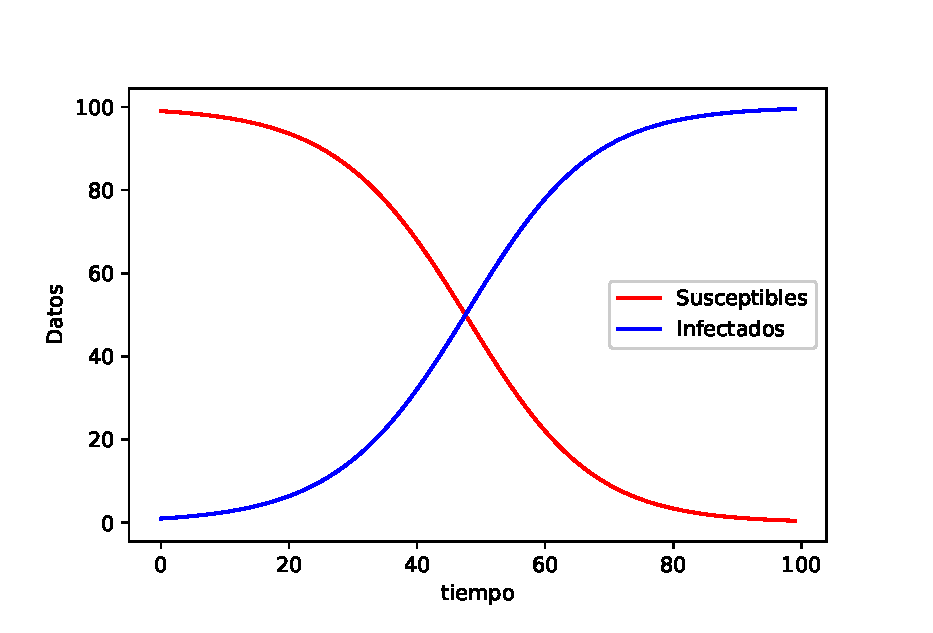
\includegraphics[scale=0.6]{graficaSI}
        \end{center}
    \end{figure}
\end{frame}


\subsection{Modelo SIR}


\begin{frame}{Modelo SIR (I)}

    \begin{block}{Modelo SIR \cite{allenDiscretetimeSISIR1994}\cite{brauerMathematicalModelsPopulation2012}\cite{salinelliDiscreteDynamicalModels2014}}
        \begin{equation}
        \label{eqn: SIR_modelo}
        \begin{aligned}
        S_{n+1} = & S_n \left(1-\frac{\alpha\Delta t}{N} I_n \right) \\
        I_{n+1} = & I_n \left( 1-\gamma \Delta t + \frac{\alpha\Delta t}{N} S_n \right) \\
        R_{n+1} = & R_n + \gamma \Delta t I_n
        \end{aligned}
        \end{equation}
        
        Con condiciones iniciales $S_0>0$, $I_0>0$, $R_0\geq 0$, satisfaciendo $S_0+I_0+R_0=N$.
    \end{block}

    \begin{center}
        \begin{tikzpicture}
            \begin{scope}[every node/.style={circle,thick,draw}]
                \node (S) at (0,0) {S};
                \node (I) at (3,0) {I};
                \node (R) at (6,0) {R};
            \end{scope}
            
            \begin{scope}[>={Stealth[black]}, every edge/.style={draw=black,very thick}]
                \path [->] (S) edge node {} (I);
                \path [->] (I) edge node {} (R);
            \end{scope}
        \end{tikzpicture}
        \end{center}

\end{frame}


\begin{frame}{Modelo SIR (II)}

        \begin{lema}
            $S_n$ es estrictamente decreciente y $R_n$ es estrictamentre creciente.
        \end{lema}

        \pause

        \begin{definicion}
            Definimos el número básico reproductivo como la constante 
            $$\mathcal{R}_{SIR}=\frac{S_0 \alpha}{N\gamma }.$$
        \end{definicion}

\end{frame}


\begin{frame}{Modelo SIR (III)}
    \begin{figure}
        \begin{center}
        \caption{Modelo SIR, $N=100$, $S_0=99$, $I_0 = 1$, $R_0 = 0$, $\alpha = 0.1$, $\gamma = 0.01$, $T_0 = 0$, $T = 300$.}
        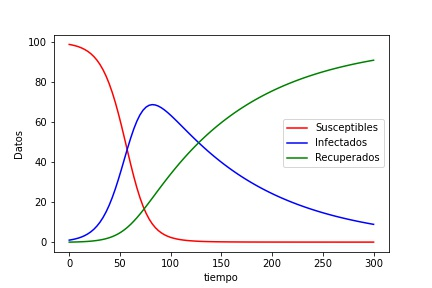
\includegraphics[scale=0.6]{graficaSIR}
        \end{center}
    \end{figure}
\end{frame}


\subsection{Modelo SIS}


\begin{frame}{Modelo SIS (I)}
    \begin{block}{Modelo SIS \cite{allenDiscretetimeSISIR1994}\cite{brauerMathematicalModelsPopulation2012}\cite{salinelliDiscreteDynamicalModels2014}}
        \begin{equation}
            \label{eqn: modelo_SIS}
            \begin{aligned}
            S_{n+1} & = S_n \left(1-\frac{\alpha\Delta t}{N} I_n \right) + \gamma \Delta t I_n \\
            I_{n+1} & = I_n \left( 1-\gamma \Delta t + \frac{\alpha\Delta t}{N} S_n \right)
            \end{aligned}
            \end{equation}
            
            Con condiciones iniciales $S_0>0$, $I_0>0$ cumpliendo $S_0+I_0=N$.
    \end{block}

    \begin{center}
        \begin{tikzpicture}
            \begin{scope}[every node/.style={circle,thick,draw}]
                \node (S) at (0,0) {S};
                \node (I) at (3,0) {I};
            \end{scope}
            
            \begin{scope}[>={Stealth[black]}, every edge/.style={draw=black,very thick}]
                \path [->] (S) edge node {} (I);
                \path [->] (I) edge[bend right=60] node {} (S); 
            \end{scope}
        \end{tikzpicture}
        \end{center}

\end{frame}


\begin{frame}{Modelo SIS (II)}

    \begin{lema}
        Los puntos de equilibrio de \eqref{eqn: modelo_SIS} son o bien $(S^*,I^*)=(N,0)$, o bien $(S^*,I^*)=(\frac{N\gamma}{\alpha}, N-\frac{N\gamma}{\alpha})$.
    \end{lema}

    \pause

    \begin{definicion}
        El número básico reproductivo se define como 
        $$\mathcal{R}_{SIS}=\frac{\alpha}{\gamma}.$$
    \end{definicion}
\end{frame}


\begin{frame}{Modelo SIS (III)}


    \begin{figure}
        \begin{center}
        \caption{Modelo SIS, $N=100$, $S_0=95$, $I_0 = 5$, $\alpha = 0.1$, $\gamma=0.01$, $T_0 = 0$, $T = 150$.}
        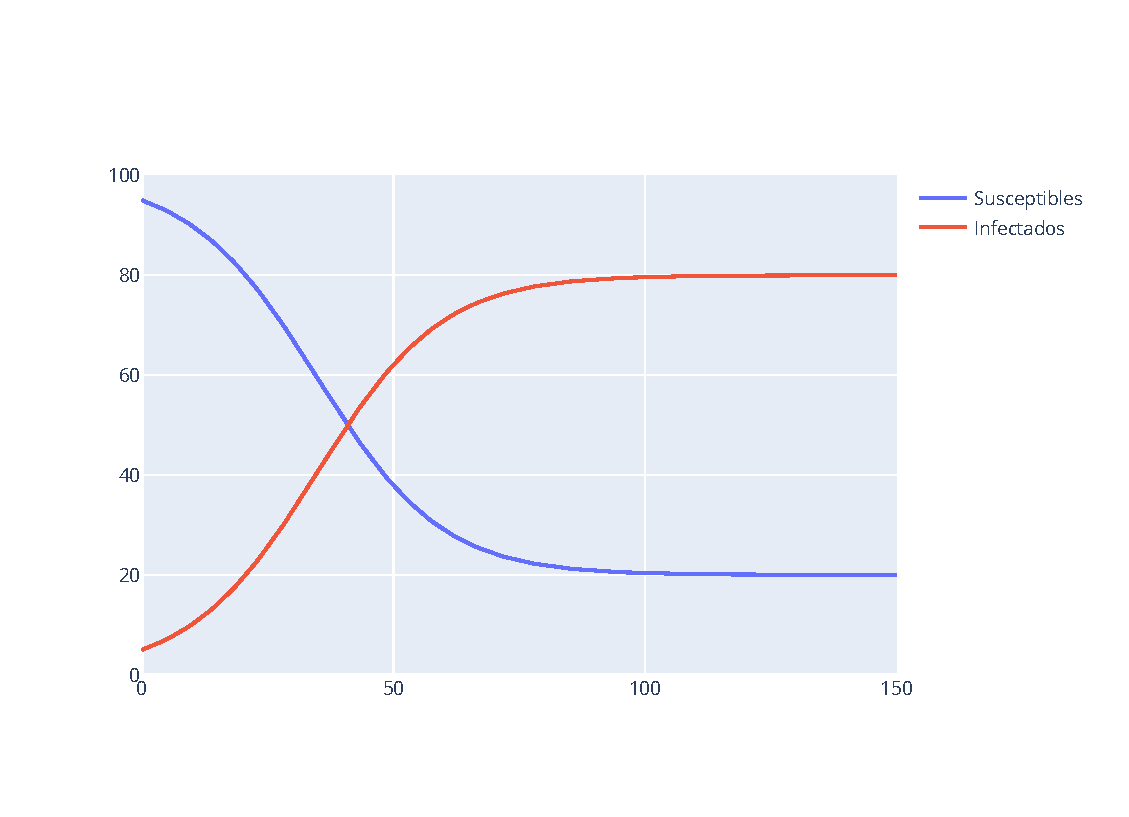
\includegraphics[scale=0.5]{SIS_modelo}
        \end{center}
    \end{figure}

\end{frame}


%%%%%%%%%%%%%%%%%%%%%%%%%%%%%%%%%%%%%%%%%%


\section{Modelos continuos en epidemiología}


\begin{frame}{Deducción del modelo continuo a partir de su análogo discreto}

    Se pueden obtener las versiones análogas continuas de los modelos discretos estudiados considerando:    
    $$\frac{S_{n+1} - S_n}{\Delta t} \approx S'(t).$$
    
    \pause
    \begin{block}{Modelo SI}
        \begin{equation}
            \label{eqn:SI_continuo}
            \begin{aligned}
            S'(t) & = -\frac{\alpha}{N}SI \\
            I'(t) & = \frac{\alpha}{N}SI
            \end{aligned}
        \end{equation}
            
        Con condiciones iniciales $S(0)+I(0)=N$.
    \end{block}
\end{frame}


\begin{frame}{Modelos SIR y SIS continuo}

    \begin{block}{Modelo SIR}
        \begin{equation}
            \label{eqn: modelo_SIR_continuo}
            \begin{aligned}
            S'(t) = & -\dfrac{\alpha}{N}SI \\
            I'(t) = & I\left(\dfrac{\alpha}{N}S-\gamma \right) \\
            R'(t) = & \gamma I
            \end{aligned}
            \end{equation}
            
            Con $S(0)+I(0)+R(0)=N$.
    \end{block}

    \pause

    \begin{block}{Modelo SIS}
        \begin{equation}
            \label{eqn: modelo_SIS_continuo}
            \begin{aligned}
            S'(t) = & -\frac{\alpha}{N}SI+\gamma I \\
            I'(t) = & I\left( \frac{\alpha}{N}S-\gamma \right) \\
            \end{aligned}
            \end{equation}
        
            Con $S(0)+I(0)=N$. 
        \end{block}
\end{frame}


%%%%%%%%%%%%%%%%%%%%%%%%%%%%%%%%%%%%%%%%%%


\section{Desarrollo del software}


\subsection{Diseño}


\begin{frame}{Diseño de la página web (I)}

    \begin{itemize}
        \item Extracción de requisitos funcionales, no funcionales y de información.
        \item Metodología de desarrollo del software: Desarrollo en espiral.

        \begin{figure}
            \begin{center}
            \caption{Modelo en espiral.}
            \label{modelo_espiral}
            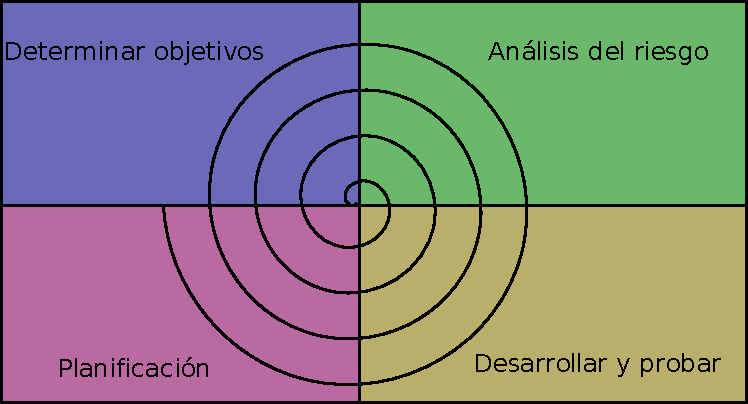
\includegraphics[scale=0.5]{modelo_espiral}
            \end{center}
            \end{figure}
    \end{itemize}

\end{frame}

\begin{frame}{Diseño de la página web (II)}

    \begin{itemize}
        \item Gestión de recursos: recursos humanos, hardware y software. Estimación del coste.
        \item Planificación temporal de las etapas del proyecto.
        \item Diagrama conceptual.
    \end{itemize}

   \begin{columns}
        \begin{column}{0.5\textwidth}  
            \begin{figure}[!h]
                \begin{center}
                \caption{Planificación temporal.}
                \label{fig: planificacion}
                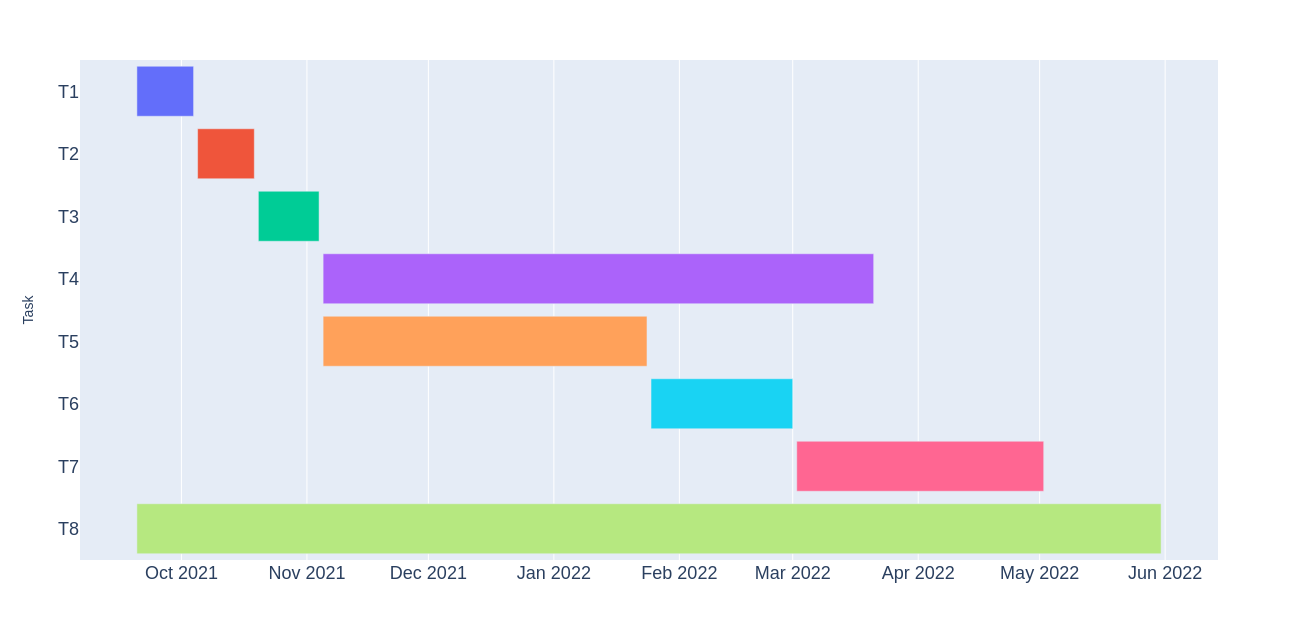
\includegraphics[scale=0.15]{planificacion}
                \end{center}
                \end{figure}
        \end{column}
    
        \begin{column}{0.5\textwidth}  
            \begin{figure}[!h]
                \begin{center}
                \caption{Modelo conceptual.}
                \label{diag: modelo_concep}
                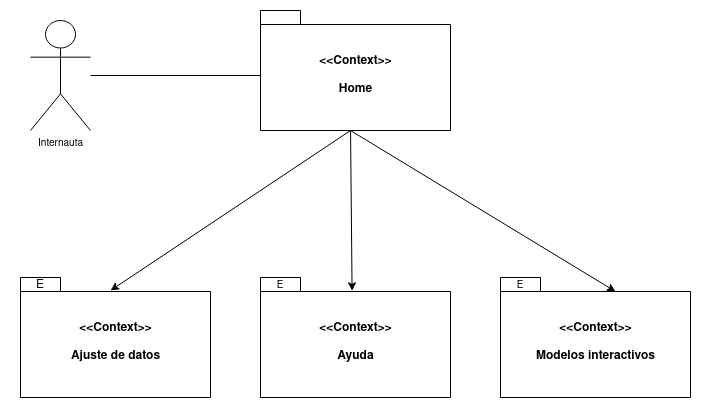
\includegraphics[scale=0.23]{modelo_conceptual-vista-paquetes.drawio}
                \end{center}
                \end{figure}
        \end{column}
\end{columns} 

\end{frame}


\begin{frame}{Diseño de la página web (III)}

    \begin{itemize}
        \item Obtención de los casos de uso.
        \item Elaboración de diagramas de actividad.
        \item Elaboración de pruebas.
        \item Diseño de la interfaz.
    \end{itemize}

    \begin{columns}
        \begin{column}{0.5\textwidth} 
            \begin{figure}[!h]
                \begin{center}
                \caption{Diagrama de casos de uso}
                \label{diag: casos_uso}
                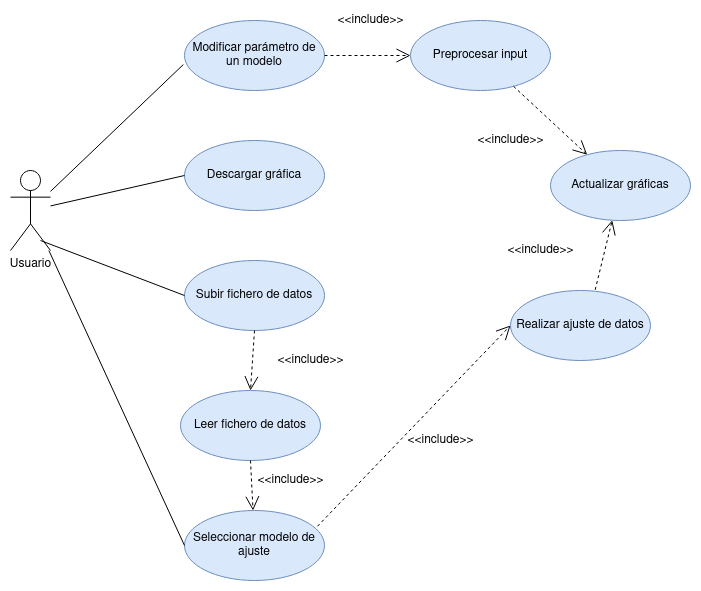
\includegraphics[scale=0.2]{casos_de_uso.drawio}
                \end{center}
                \end{figure}
        \end{column}
    
        \begin{column}{0.5\textwidth}  
            \begin{figure}[!h]
                \begin{center}
                \caption{Plantilla de un caso de uso.}
                \label{diag: plantilla_cu}
                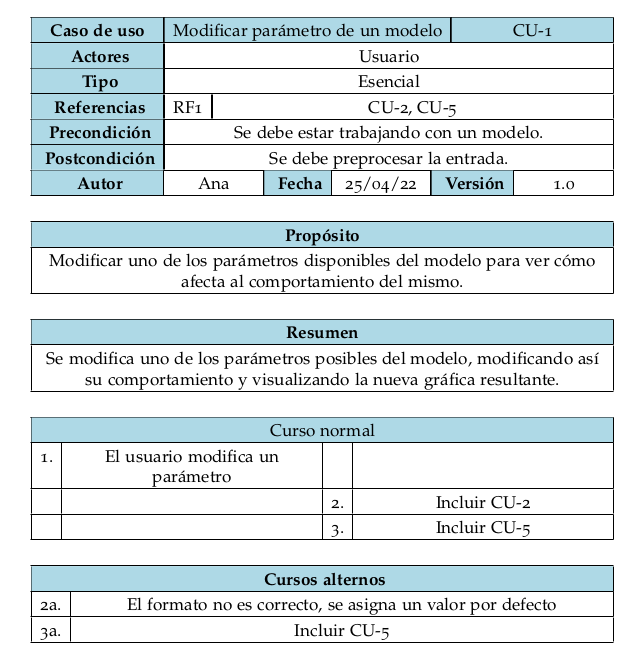
\includegraphics[scale=0.2]{plantilla_cu}
                \end{center}
                \end{figure}
        \end{column}
    \end{columns}

\end{frame}



\subsection{Demostración de uso}


\begin{frame}{Herramientas y demostración de uso}

    \begin{itemize}
        \item Gráficas interactivas $\Rightarrow$ Dash \cite{dash}.
        \pause
        \item Framework para la web $\Rightarrow$ Flask \cite{flask}.
        \pause
        \item Virtualización $\Rightarrow$ Docker \cite{docker}.
        \pause
        \item Control de versiones y repositorio $\Rightarrow$ Git y Github \cite{git}.
        \begin{itemize}
            \item \href{https://github.com/Mapachana/TFG}{https://github.com/Mapachana/TFG}
        \end{itemize}
        \pause
        \item Ajuste de datos $\Rightarrow$ Scipy \cite{scipy_curvefit}.
        \begin{itemize}
            \item Ajuste por mínimos cuadrados.
            \item Estimación de parámetros.
            \item Expresión de los errores como 1/(1+MSE).
            \item Selección del modelo con mínimo error para unos datos dados.
        \end{itemize}
    \end{itemize}

    \pause

    \href{run:./demo_plotsir.mkv}{Demostración de uso de la página.}

\end{frame}


\subsection{Estimación de parámetros en datos reales}


\begin{frame}{El VIH en Baleares}

    \begin{figure}
        \begin{center}
        \caption{Ajuste con el modelo SI a los datos del VIH en Baleares \cite{datos_vih}.}
        \label{ajuste_vih}
        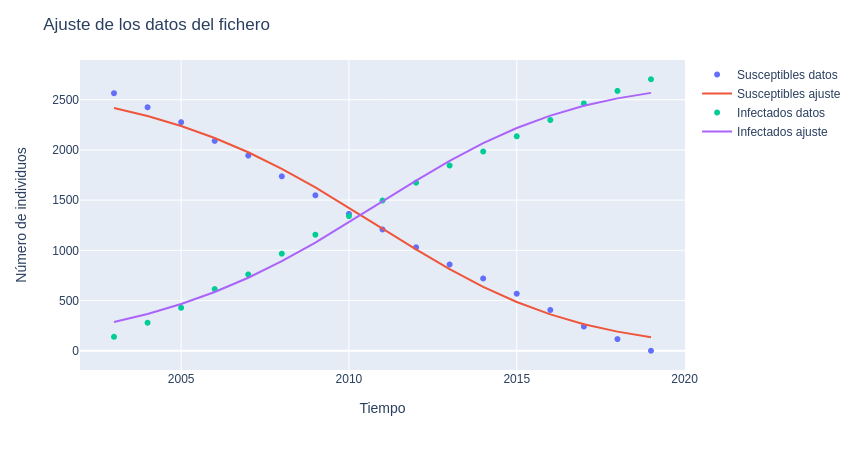
\includegraphics[scale=0.35]{ajuste_vih}
        \end{center}
        \end{figure}
\end{frame}


\begin{frame}{El Covid-19 en España}
    \begin{figure}
        \begin{center}
        \caption{Ajuste con el modelo SIR a los datos del Covid-19 en España desde el 5 de Marzo hasta el 21 de Agosto de 2020 \cite{datos_covid}.}
        \label{ajuste_covid}
        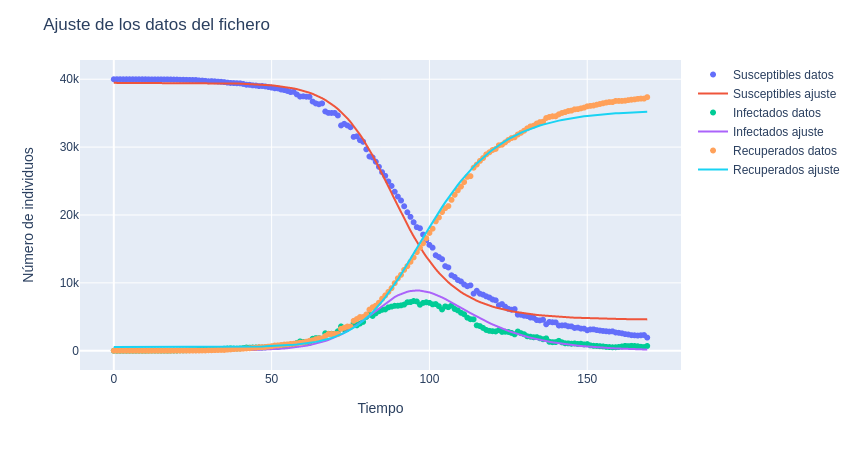
\includegraphics[scale=0.35]{ajuste_covid}
        \end{center}
        \end{figure}


\end{frame}


%%%%%%%%%%%%%%%%%%%%%%%%%%%%%%%%%%%%%%%%%%


\section{Conclusiones}


\begin{frame}{Conclusiones}

    \begin{itemize}
        \item Estos modelos presentan muchas limitaciones, ya que se usan suposiciones que rara vez ocurren en casos reales.
        \item Los datos reales presentan ruido e incompletitud.
        \item Se pueden mejorar los modelos añadiendo más estados.
        \item Los modelos presentados son una herramienta muy potente y útil pese a todas las limitaciones encontradas.
    \end{itemize}

\end{frame}


%%%%%%%%%%%%%%%%%%%%%%%%%%%%%%%%%%%%%%%%%%


\begin{frame}{Referencias}
    \bibliography{../redaccion_tfg/bib/library.bib}
    \bibliographystyle{plain}
\end{frame}


{

\usebackgroundtemplate{ \parbox[b][\paperheight][b]{\paperwidth}{\centering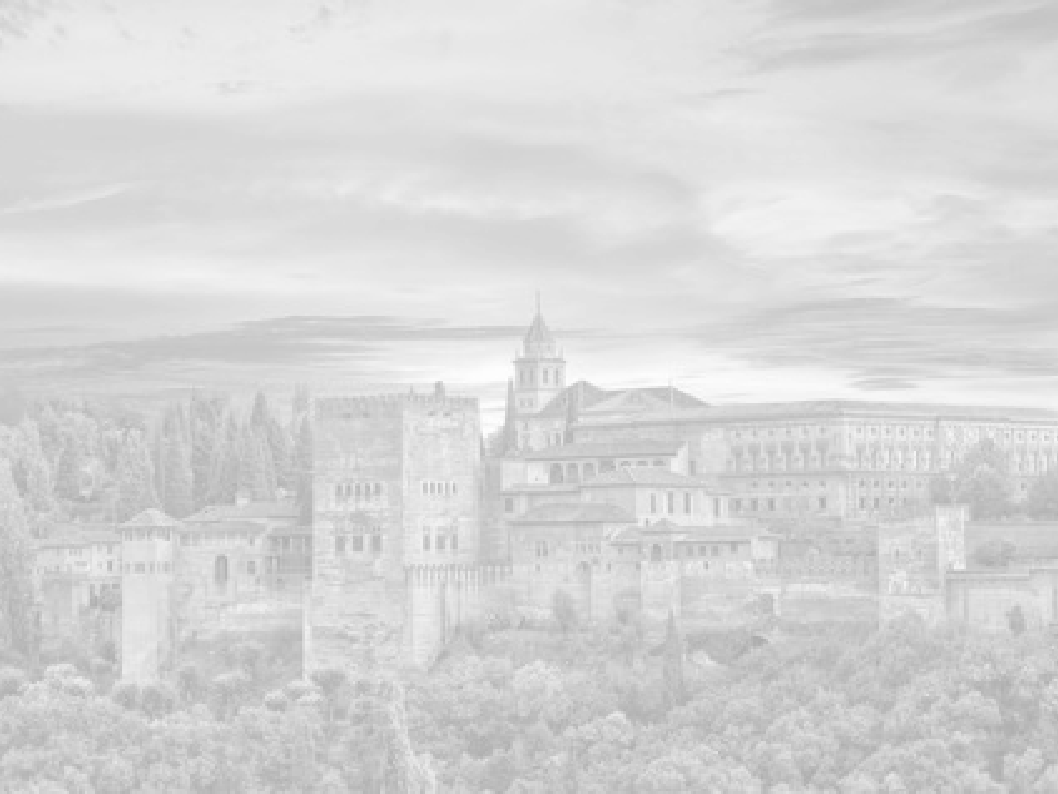
\includegraphics[width=\paperwidth]{Background/bg_alhambra.png}}} 

\title[Gracias por su atención]{Gracias por su atención.}
\subtitle{}
\author{}
\institute{}
\date{}
\begin{frame}[plain,noframenumbering]
    \titlepage
\end{frame}

}	
